\chapter{Adversarial Tracking}
\label{chpt:tracking}

% \newrefsection

In this chapter, we present adversarial attacks against object tracking systems. Unlike object detection systems that only make predictions based on the current input image from the camera, object tracking models combine prior predictions with current inputs to generate trajectories of moving objects, making them more robust to adversarial attacks.

\section{Introduction}
\label{sec:adv_track}

As introduced in Chapter \ref{chpt:driving}, deep learning models are widely used in autonomous driving for perception tasks, such as object-tracking, to generate trajectories of surrounding vehicles. In this context, we lack access to gradients, which makes white-box attacks nearly impossible. Additionally, the difficulty in obtaining intermediate query results within the internal data path makes it impractical for black-box attacks to query the model.

However, this does not necessarily mean that current autonomous driving systems are robust against adversarial attacks. Many object tracking systems still rely on pre-trained object detection models (as outlined in Table \ref{tab.detection_github}), making them susceptible to transferable perturbations generated using well-known object detection models. Consequently, adversarial attacks targeting object detection could also impact object tracking systems.

\begin{table}[H]
\centering
\begin{tabular}{ ccc } 
\hline
Rank & Model & Popularity \\
\hline
1 & SSD & 605 \\ 
2 & YOLO-v3 & 251 \\ 
3 & Faster R-CNN & 236 \\ 
4 & R-CNN & 178 \\ 
5 & YOLO-v2 & 164 \\ 
6 & RetinaNet & 75 \\ 
7 & Yolo-v1 & 52 \\ 
\hline
\end{tabular}
\caption{Most popular object detection models on GitHub \citep{wang2021daedalus}}
\label{tab.detection_github}
\end{table}

% In the next step, we plan to implement a real-time object tracking system. Then we can investigate the effect of hardware acceleration on the robustness of the model, and if it's possible to attack such a system without prior knowledge of the structure of the model.

\subsection{Object Tracking}

The first tracking system used radar and sonar to track objects for military applications, and the algorithm consists of four parts: data association, state update, state prediction, and track management. Later, the employment of deep learning yields significant performance increases for visual tracking tasks.

Before the widespread adoption of deep learning, visual tracking problems were commonly addressed using low-level features and statistical learning techniques. These included methods such as the Joint Probabilistic Data Association Filter (JPDAF), Multi-Hypothesis Tracking (MHT), and Random Finite Sets (RFS). These techniques were often combined with nonlinear filters such as Bayesian Estimation, the Kalman Filter, the Particle Filter, and the Gaussian Sum Filter to establish correspondences between detections and tracklets \citep{vo2015multitarget}. 

As research in deep learning advances, traditional low-level features and statistical learning techniques for object tracking are being replaced by deep neural networks. Deep neural networks are widely utilized for both \acrfull{sot} and \acrfull{mot} applications \citep{krebs2017survey}.

\textbf{\acrfull{sot}} focuses on tracking one specified target within a sequence of input image frames. The target can be specified using a template image or be chosen from the first frame \citep{soleimanitaleb2022single} (see Fig. \ref{fig:sot}). Similar to face recognition, the image of a target person may not appear in the training set, so the SOT model must be capable of tracking any given object with only one image. Besides, the class label may not be available in the training set, requiring the model to handle a variety of potential targets.

\acrshort{sot} commonly uses a Siamese network to learn a similarity function that differentiates objects and then utilizes statistical methods to update and maintain a single tracklet effectively \citep{he2018twofold, guo2017learning, bertinetto2016fully, dong2018triplet, zhang2019deeper}.

\textbf{\acrfull{mot}}, in contrast, involves tracking multiple objects simultaneously and maintaining multiple tracklets. In MOT, the number of classes is typically predefined, and the tracking model assigns a unique ID to each detected object. The primary challenge in MOT is differentiating distinct objects and associating the same object across consecutive frames to maintain consistent tracklets (see Fig. \ref{fig:mot}).

% Image Classification: Classify the most salient object of the entire image.

% Object Detection: Classify and Detection the position of each object. (more challenging than classification). We detect the object independently in each frame.

% Object Tracking: Classify and Detect the position of each object as well as estimating the motion model of each object (more challenging than detection).

% Hungarian method was used to find the optimal association to an assignment problem in 2008.

\begin{figure}[t]
    \centering
    \begin{subfigure}[b]{0.38\textwidth}
        \centering
        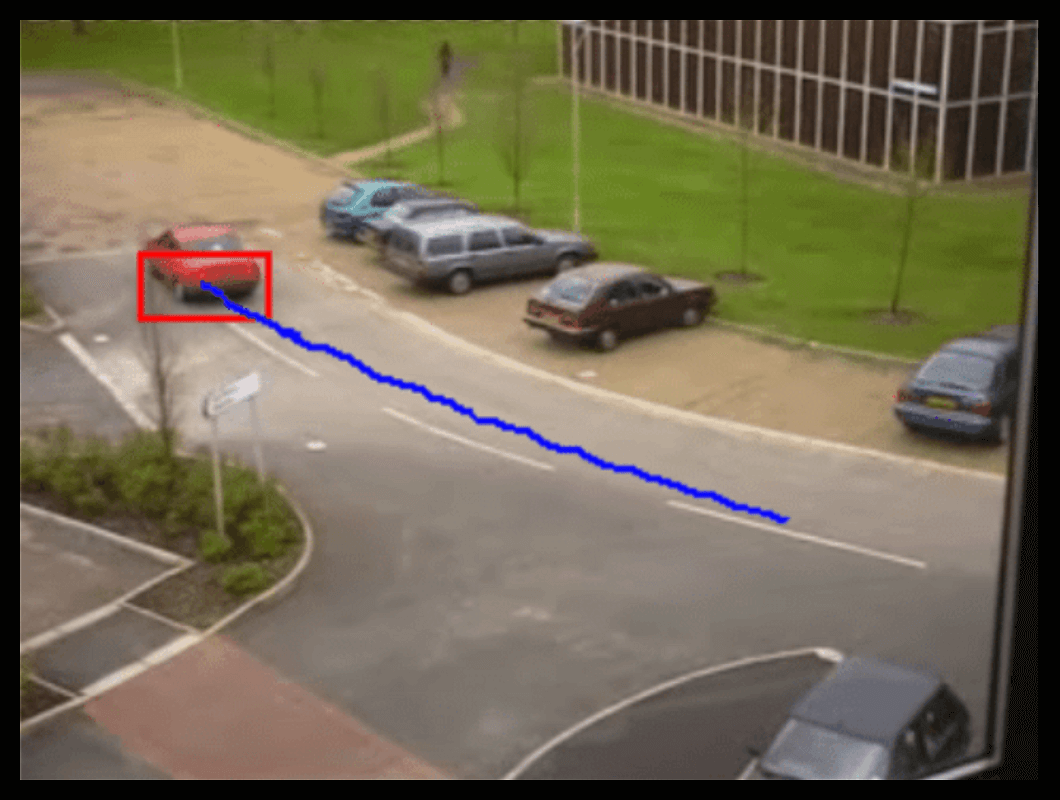
\includegraphics[width=\linewidth]{figures/chapter_tracking/sot.png}
        \caption{\acrshort{sot} }
        \label{fig:sot} 
    \end{subfigure}
    \begin{subfigure}[b]{0.61\textwidth}
        \centering
        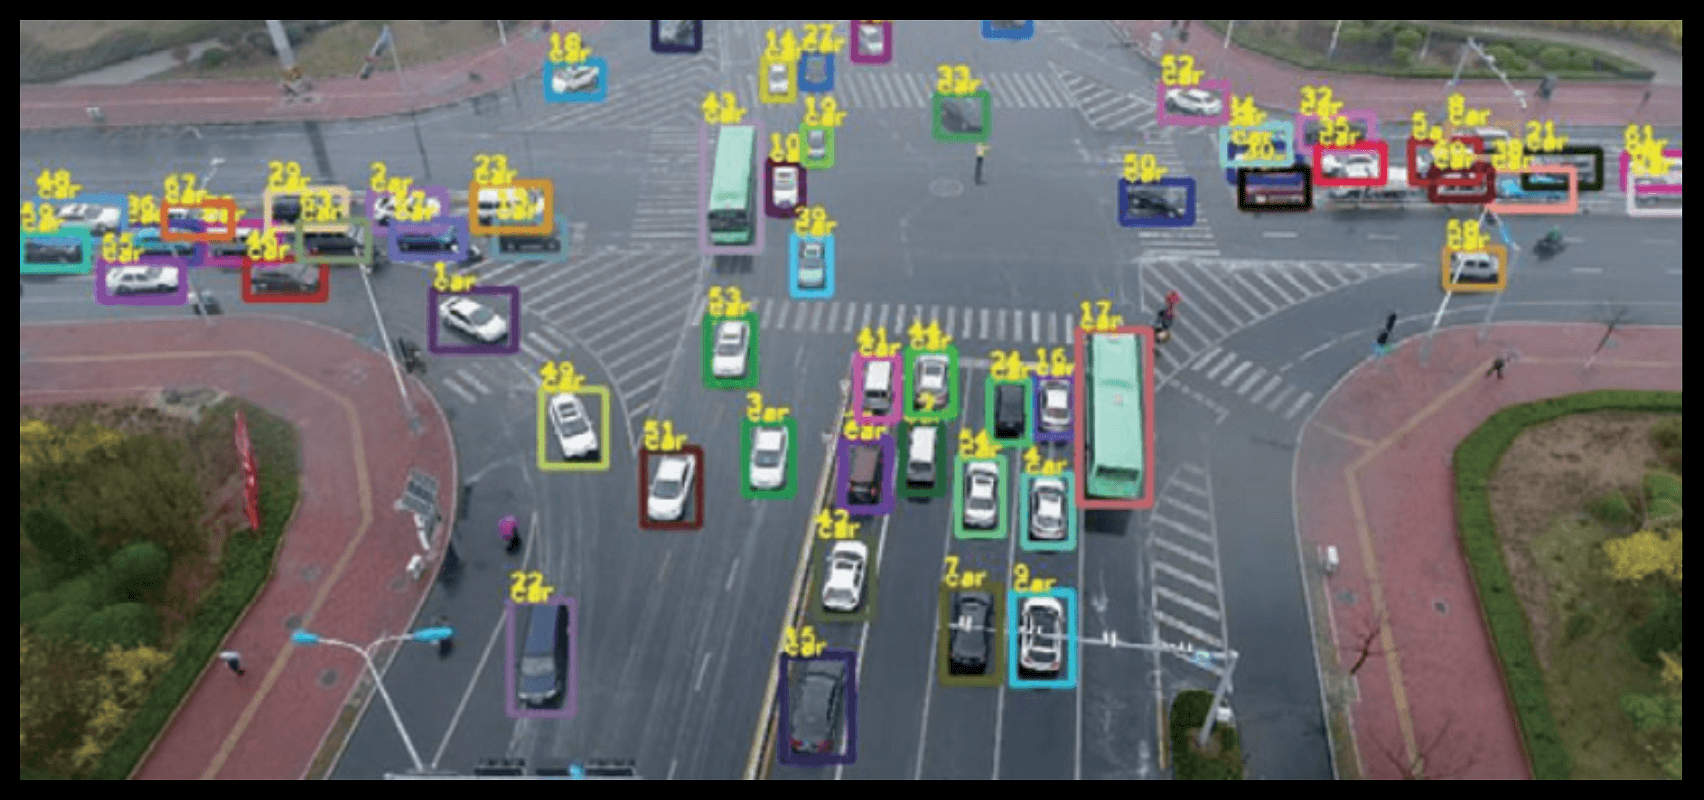
\includegraphics[width=\linewidth]{figures/chapter_tracking/mot.png}
        \caption{\acrshort{mot}}
        \label{fig:mot}
    \end{subfigure}
  \caption{The difference between \acrfull{sot} \citep{jansari2013real} and \acrfull{mot} \citep{liu2022multi}.}
  \label{fig:tracking}
\end{figure}

Recent research interests are shifting from \acrshort{sot} to \acrshort{mot}, especially in the context of autonomous driving, which demands a comprehensive perception of surrounding vehicles. Table \ref{tab.mot} highlights the top-performing methods on the KITTI multi-object tracking leaderboard for autonomous driving \citep{Geiger2012CVPR}.

\begin{table}[t]
\centering
\begin{tabular}{ lcccc } 
\hline
Method & Sensor & Type & Real-Time & HOTA    \\
\hline
BiTrack (Not publications yet) &    Lidar   &      -         & N & 82.69\% \\ 
LEGO \citep{zhang2023lego}   &    Lidar   &      -         & Y  & 80.75\% \\ 
CollabMOT \citep{ninh2024collabmot}   &    Stereo   &      \acrshort{tbd}         & N  & 80.02\% \\ 
RAM \citep{tokmakov2022object}    &    Mono  & \acrshort{jdt} & Y  & 79.53\% \\ 
PermaTrack \citep{tokmakov2021learning} & Mono  & \acrshort{jdt} & Y  & 78.03\% \\ 
\textbf{OC-SORT \citep{cao2023observation}}    & \textbf{Mono}  & \textbf{\acrshort{tbd}} & \textbf{Y}  & \textbf{76.54\%} \\ 
\hline
\end{tabular}
\caption{Top \acrfull{mot} methods on the KITTI leaderboard.}
\label{tab.mot}
\end{table}

\subsubsection{Object Tracking Sensors}

Camera and Lidar are the two most popular sensors used in autonomous vehicles. On the KITTI leaderboard, the method that utilizes point clouds from a Velodyne laser scanner achieves the highest Higher Order Tracking Accuracy (HOTA) \citep{Luiten2020IJCV}. We introduce the \acrshort{hota} evaluation metric in Sec. \ref{sec:tracking_eval}.

\textbf{Monocular Tracker}:  Vision-only methods rely solely on input images from a single camera \citep{wu2021track} \citep{hu2022monocular} are accurate for 2D multi-object tracking. However, they cannot reliably predict 3D locations because depth information is absent from single-camera input.

\textbf{Binocular Tracker}: This approach combines 2D object detection results with depth information obtained from stereo vision to achieve 3D object detection and tracking. However, using a stereo camera setup requires extensive calibration and complex matching algorithms \citep{ninh2024collabmot}.

\textbf{Multi-Modality Tracker}: Accurately estimating vehicles' pose in 3D space is crucial for autonomous driving. By combining 2D detection results with 3D Lidar data, this approach achieves the highest tracking accuracy on the KITTI leaderboard, though at the cost of using more expensive 3D laser scanners than CMOS cameras.

% \clearpage

\subsubsection{Object Tracking Frameworks}

\acrfull{tbd} and \acrfull{jdt} are the two most popular frameworks for object tracking applications.

\textbf{\acrfull{tbd}} is a modular object tracking framework that consists of object localization, feature extraction, data association, and track management (see Fig. \ref{fig:tbd}). Object detection models handle object localization and feature extraction to generate bounding boxes, while traditional methods such as the Hungarian Algorithm manage data association, and the Kalman Filter oversees track management. The overall accuracy of the TBD framework depends significantly on the precision of the detector, such as SiamRPN++ \citep{li2019siamrpn++} for \acrshort{sot} and YOLO, Faster R-CNN, and SSD for \acrshort{mot} applications \citep{sun2020survey}.

\textbf{\acrfull{jdt}}: As more accurate and efficient deep neural networks, such as Vision Transformer \citep{dosovitskiy2020image}, are being developed, there is also a growing trend of employing end-to-end tracking models \citep{pal2021deep, guo2022review}. PermaTrack is a \acrshort{jdt} method that takes multiple frames of images as input and outputs the position and velocity of each vehicle (see Fig. \ref{fig:jdt}). As can be seen from Tab. \ref{tab.mot}, \acrshort{jdt} methods achieve slightly higher accuracy than \acrshort{tbd} methods.

% \item Transformer: More accurate, but computationally expensive \citep{meinhardt2022trackformer} for 2D MOT \citep{lin2021swintrack}.

To explore whether traditional statistical methods, such as the Kalman Filter, can help mitigate the impact of adversarial attacks, we focus on modular \acrshort{tbd} methods (highlighted in Tab \ref{tab.mot}) instead of end-to-end \acrshort{jdt} models. Additionally, due to the lower cost and ease of setup of monocular cameras compared to 3D Lidar and stereo cameras, our primary focus is on vision-only monocular 2D object detection.

% Object Tracking Assumptions: 

% \begin{enumerate}
%     \item Camera is not moving instantly to new viewpoint.
%     \item Objects do not disappear and reappear in different places in the scene.
%     \item If the camera is moving, there is a gradual change in pose between camera and scene.
% \end{enumerate}

\begin{figure}[H]
    \centering
    \begin{subfigure}[b]{\textwidth}
        \centering
        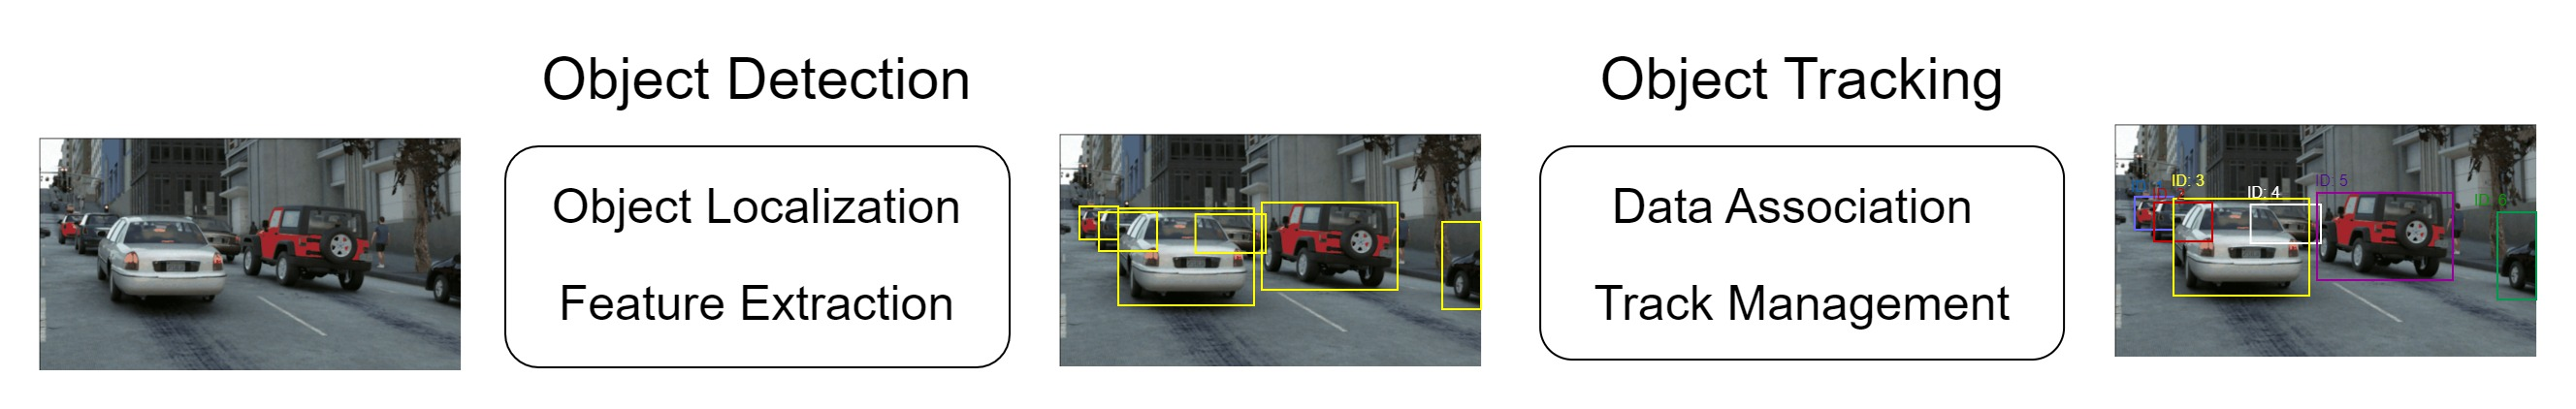
\includegraphics[width=\linewidth]{figures/chapter_tracking/tbd.jpg}
        \caption{\acrlong{tbd} (Modular System)}
        \label{fig:tbd} 
    \end{subfigure}
    \begin{subfigure}[b]{\textwidth}
        \centering
        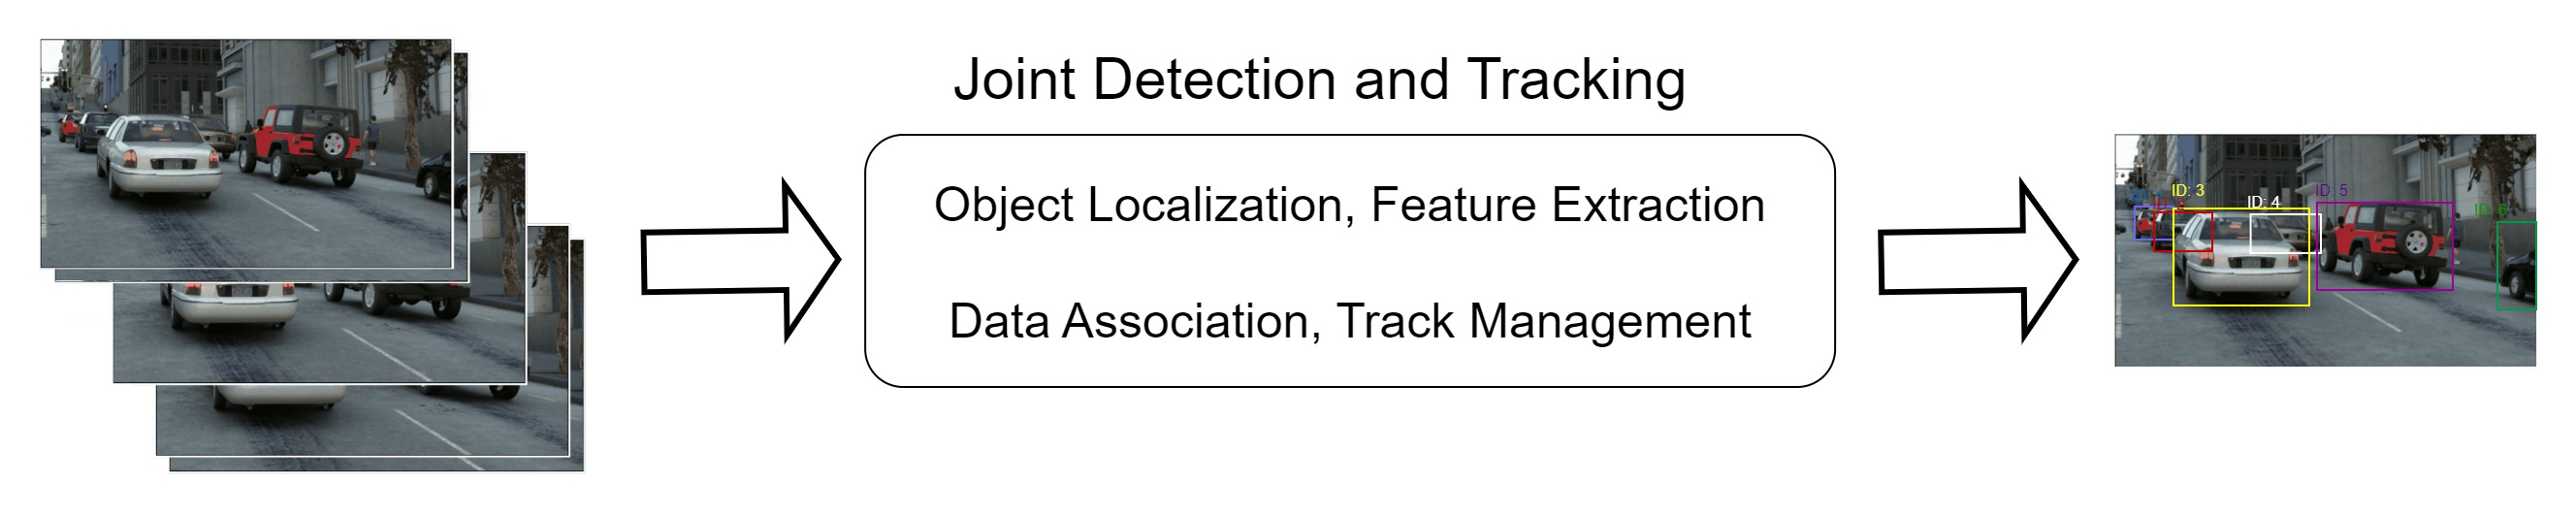
\includegraphics[width=\linewidth]{figures/chapter_tracking/jdt.jpg}
        \caption{\acrlong{jdt} (End-to-End Model)}
        \label{fig:jdt}
    \end{subfigure}
  \caption{The difference between \acrfull{tbd} and \acrfull{jdt}.}
  \label{fig:tracking_framework}
\end{figure}

% \clearpage

\subsection{Adversarial Attacks}

Adversarial attacks have progressed from image classification to object detection and then object tracking models. Notably, \acrfull{jdt} methods that utilize end-to-end deep learning models, such as GOTURN \citep{wiyatno2019physical} and FairMOT \citep{lin2021trasw}, are vulnerable to adversarial attack. For \acrfull{tbd} methods, adversaries focus on vulnerabilities in various components within the tracking system, including the object detector, the association method, and the tracklet management module.

\textbf{Attacking Object Detectors}: The accuracy of \acrshort{tbd} methods heavily relies on the object detector's ability to produce precise bounding boxes of target objects. If the object detector produces bounding boxes at incorrect positions or does not predict bounding boxes at all, the subsequent modules will struggle to generate precise tracklets. 

Table \ref{tab.mot_attack} presents studies focusing on attacking object detectors, and most work attacks SiameseRPN-based trackers  \citep{wu2019sta}. Siamese neural networks employ triplet loss or contrastive loss to train a similarity function to discern objects, such as distinguishing facial features in face recognition systems. 

In 2019, the first adversarial attack against \acrshort{mot} models attacked a \acrshort{tbd} method that used YOLOv3 as the object detector \citep{jia2020fooling}. Moreover, YOLOX \citep{ge2021yolox} and CenterNet \citep{duan2019centernet} stand out as two widely-used object detectors for autonomous driving applications, yet they both exhibit vulnerability to adversarial attacks \citep{zhou2023f,pang2024blinding}.

\textbf{Attacking Association Methods}: Another crucial factor for \acrshort{mot} system is to assign a unique ID to each detected object. It is possible to perturb the association module so that the same object may be given different IDs in different frames, thus breaking the continuity of tracklets. Liu et al. introduced the Blind Attack, which assigns the background label to the target object, and the Blur Attack, which assigns other labels to the target object \citep{liu2022efficient}.


\textbf{Attacking Tracklets}: Tracklets, commonly managed by the Kalman Filter, store the position and velocity of each vehicle. By perturbing objects' speed and direction, incorrect states are predicted for each object, enabling the switching of tracklets between adjacent objects. For instance, Lin et al. perturbed the appearance and distance similarity of two adjacent pedestrians, causing FairMOT and ByteTrack models to fail to track the targets in the subsequent frames \citep{lin2021tracklet}.

While it is acknowledged that \acrshort{mot} systems utilizing 3D Lidar Point Clouds are also susceptible to adversarial attacks \citep{cheng2021universal, cheng2022non, wang2022adversary}, our research focuses on attacks targeting vision-only \acrshort{mot} systems.

\clearpage

\begin{sidewaystable}
\centering
\begin{tabular}{ clccccc } 
\hline
Year & Method & Tracking & Model & Attack Type & Patch / Filter \\
\hline
2019 & Hijacking Attack \citep{jia2020fooling} & MOT & Yolov3 & Whitebox & Digital Patch \\
2019 & EOT Attack \citep{wiyatno2019physical} & SOT & GOTURN & Whitebox & Physical Patch \\
2020 & SPARK Attack \citep{guo2020spark} & SOT & SiamRPN++  & Whitebox & Digital Filter  \\
2020 & One-Shot Attack \citep{chen2020one} & SOT & Siamese Tracker  & Whitebox & Digital Filter \\
2020 & FAN Attack \citep{liang2020efficient} & SOT & Siamese Network & Whitebox & Digital Filter  \\
2020 & Hijacking Tracker \citep{yan2020hijacking}& SOT & SiamRPN & Whitebox & Digital Filter \\
2020 & Cool-Shrink Attack \citep{yan2020cooling} & SOT & SiamRPN++ & Whitebox & Digital Filter \\
2021 & Tracklet-Switch Attack \citep{lin2021tracklet} & MOT & FairMOT \& ByteTrack & Whitebox & Digital Filter \\
2021 & MTD Attack \citep{ding2021towards} & SOT & SiamRPN++  & Whitebox & Physical Patch \\
2021 & ABA Attack \citep{guo2021learning} & SOT & SiamRPN++ & Whitebox & Digital Blurry \\
2021 & IoU Attack \citep{jia2021iou} & SOT & SiamRPN++ & Blackbox & Digital Filter  \\
2022 & Few-Shot Attack \citep{li2022few} & SOT & SiamFC++  & Whitebox & Physical Patch\\
2022 & Ad2 Attack \citep{fu2022ad} & SOT & SiamAPN & Whitebox & Digital Filter \\
2022 & Shuffle Attack \citep{liu2022efficient} & SOT & Yolov3 + Kalman & Whitebox & Digital Filter  \\
2022 & Diminishing \citep{suttapak2022diminishing} & SOT & SiamRPN++ & Whitebox & Digital Filter    \\
2023 & F\&F Attack \citep{zhou2023f} & MOT & YOLOX \& CenterNet & Whitebox & Digital Filter  \\
2024 & Blinding \& Blurring Attack \citep{pang2024blinding} & MOT & YOLOX \& CenterNet & Whitebox & Digital Filter \\
\hline
\end{tabular}
\caption{Adversarial Attacks against Object Tracking Models.}
\label{tab.mot_attack}
\end{sidewaystable}

\clearpage

\section{Methodology}

\subsection{Problem Formulation}


\clearpage

\subsection{Evaluation metrics}
\label{sec:tracking_eval}

SORT, DeepSORT, OC-SORT (Kalman Filter)

In \citep{ciaparrone2020deep}, Ciaparrone et al. listed the most popular evaluation dataset (MOTChallenge, KITTI, nuScenes) and evaluation metrics (MOTA, MOTP, MT, ML, FP, FN).

\clearpage

\section{Experimental Results}

\subsection{Image-Specific}


\clearpage

\subsection{Image-Agnostic}

\clearpage

\section{Summary}

% In summary, we find several research papers that attack 2D SOT (caemera) and 3D MOT ( Lidar). But we do not find attacks against 3D monocular trackers \citep{wu2021track} \citep{hu2022monocular}. Neither do we find research that attacks Transformers for 2D MOT.

% We plan to attack 3D MOT models for Vision-Based vehicle tracking in real time (no 3D Lidar Data). First, we'll implement two 3D MOT models: \href{https://github.com/SysCV/qd-3dt}{QD-3DT} and \href{https://github.com/JialianW/TraDeS}{TraDeS}. Then, we'll try to design white-box attacks to fabricate, vanish 3D bounding boxes, change their orientations, or dissociate them with actual objects.

% \clearpage

% \printbibliography[
%   keyword={chapter_tracking}, heading=subbibintoc, resetnumbers=true
% ]